\subsection{Interfaz de la Aplicación}

\par
Al inicio de la aplicación mostraremos una animación con el logo y el eslogan de la compañia. El tiempo de duración de esta animación es de 2 segundos y se ejecutara siempre y cuando la aplicación no entre en el segundo plano del sistema operativo. La imagen de la animación es la siguiente:

\begin{figure}[H]
	\centering
	
\includegraphics[width=0.2\linewidth]{interfaz1.png}
	\caption{Animación de inicio de la aplicación; también conocido como "Splash Screen"}
\end{figure}

\par \noindent
Transcurridos los 2 segundos de la animación automáticamente es reemplazado por la actividad principal.  

\subsubsection{Actividad Principal}

\begin{figure}[H]
	\centering
	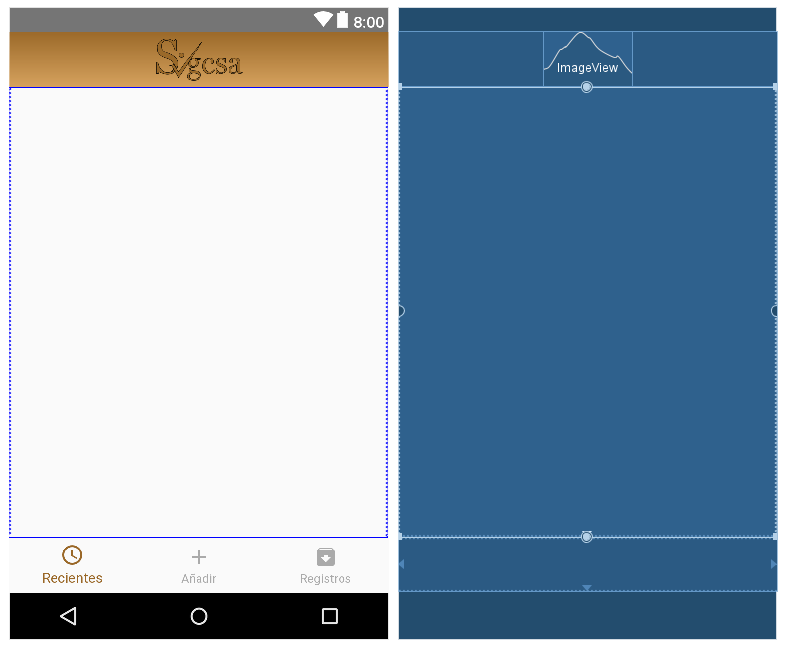
\includegraphics[width=0.8\linewidth]{interfaz2.png}
	\caption{Interfaz de la actividad principal}
\end{figure}

\par 
Pero ¿Qué es una actividad? y ¿Porqué es la actividad principal? Según la documentación oficial de Android una actividad se define como: un componente de aplicación que proporciona una pantalla con la que los usuarios pueden interactuar para hacer algo, como marcar el teléfono, tomar una foto, enviar un correo electrónico o ver un mapa. Una actividad puede iniciar otras actividades, incluidas actividades que viven en aplicaciones separadas.\cite{androidapp}

\par \noindent
Se ha llamado la actividad principal porque es donde el usuario final interactua con el resto de los componentes de la aplicación tales como menus, actividades, fragmentos y servicios. 

\par \noindent
En la imagen 4.10 podemos apreciar los 3 componentes de la actividad principal. En la parte superior se encuentra el "toolbar", su objetivo es el de mostrar información relativa a la actividad donde se encuentra; por lo que, hemos elegido utilizar el logo de la compañia SIGCSA para enfatizar que es la actividad principal. 

\par \noindent
En la parte inferior nos encontramos con una tendencia en la navegación de la aplicación moviles hoy en día. En android es llamado "BottomNavigationView", como su nombre lo indica es el encargado del manejo de las distintas fragmentos o subinterfaces utilizadas en una aplicación móvil. Es una cinta con el color de fondo de la aplicación en ella se encuentran botones que incluyen el texto y una pequeña imagen. Al seleccionar uno de estos botones la interfaz cambia con la excepción del "toolbar" y el "BottomNavigationView"; adicional el botón seleccionado incrementa ligeramente su tamaño y toma un color distinto al resto de los botones para indicar la interfaz activa en ese momento.

\par \noindent
El ultimo componente de la interfaz de la actividad principal no es visible para el usuario; sin embargo, se puede ver el borde azul en la imagen 4.10. Este componente es un "layout", en el es donde se pueden colocar otros componentes como botones, texto y más. Actúa realmente como un contenedor de componentes. En la actividad principal se encuentra vacio debido a que al iniciar la actividad debemos reemplazar este "layout" por una subinterfaz o fragmento. Por ende este componente es donde son expuestos los fragmentos seleccionados por el "BottonNavigationView" y nosotros hemos programado que el fragmento por defecto al iniciar esta actividad es el fragmento recientes.

\subsubsection{Fragmento Recientes}

\begin{figure}[H]
	\centering
	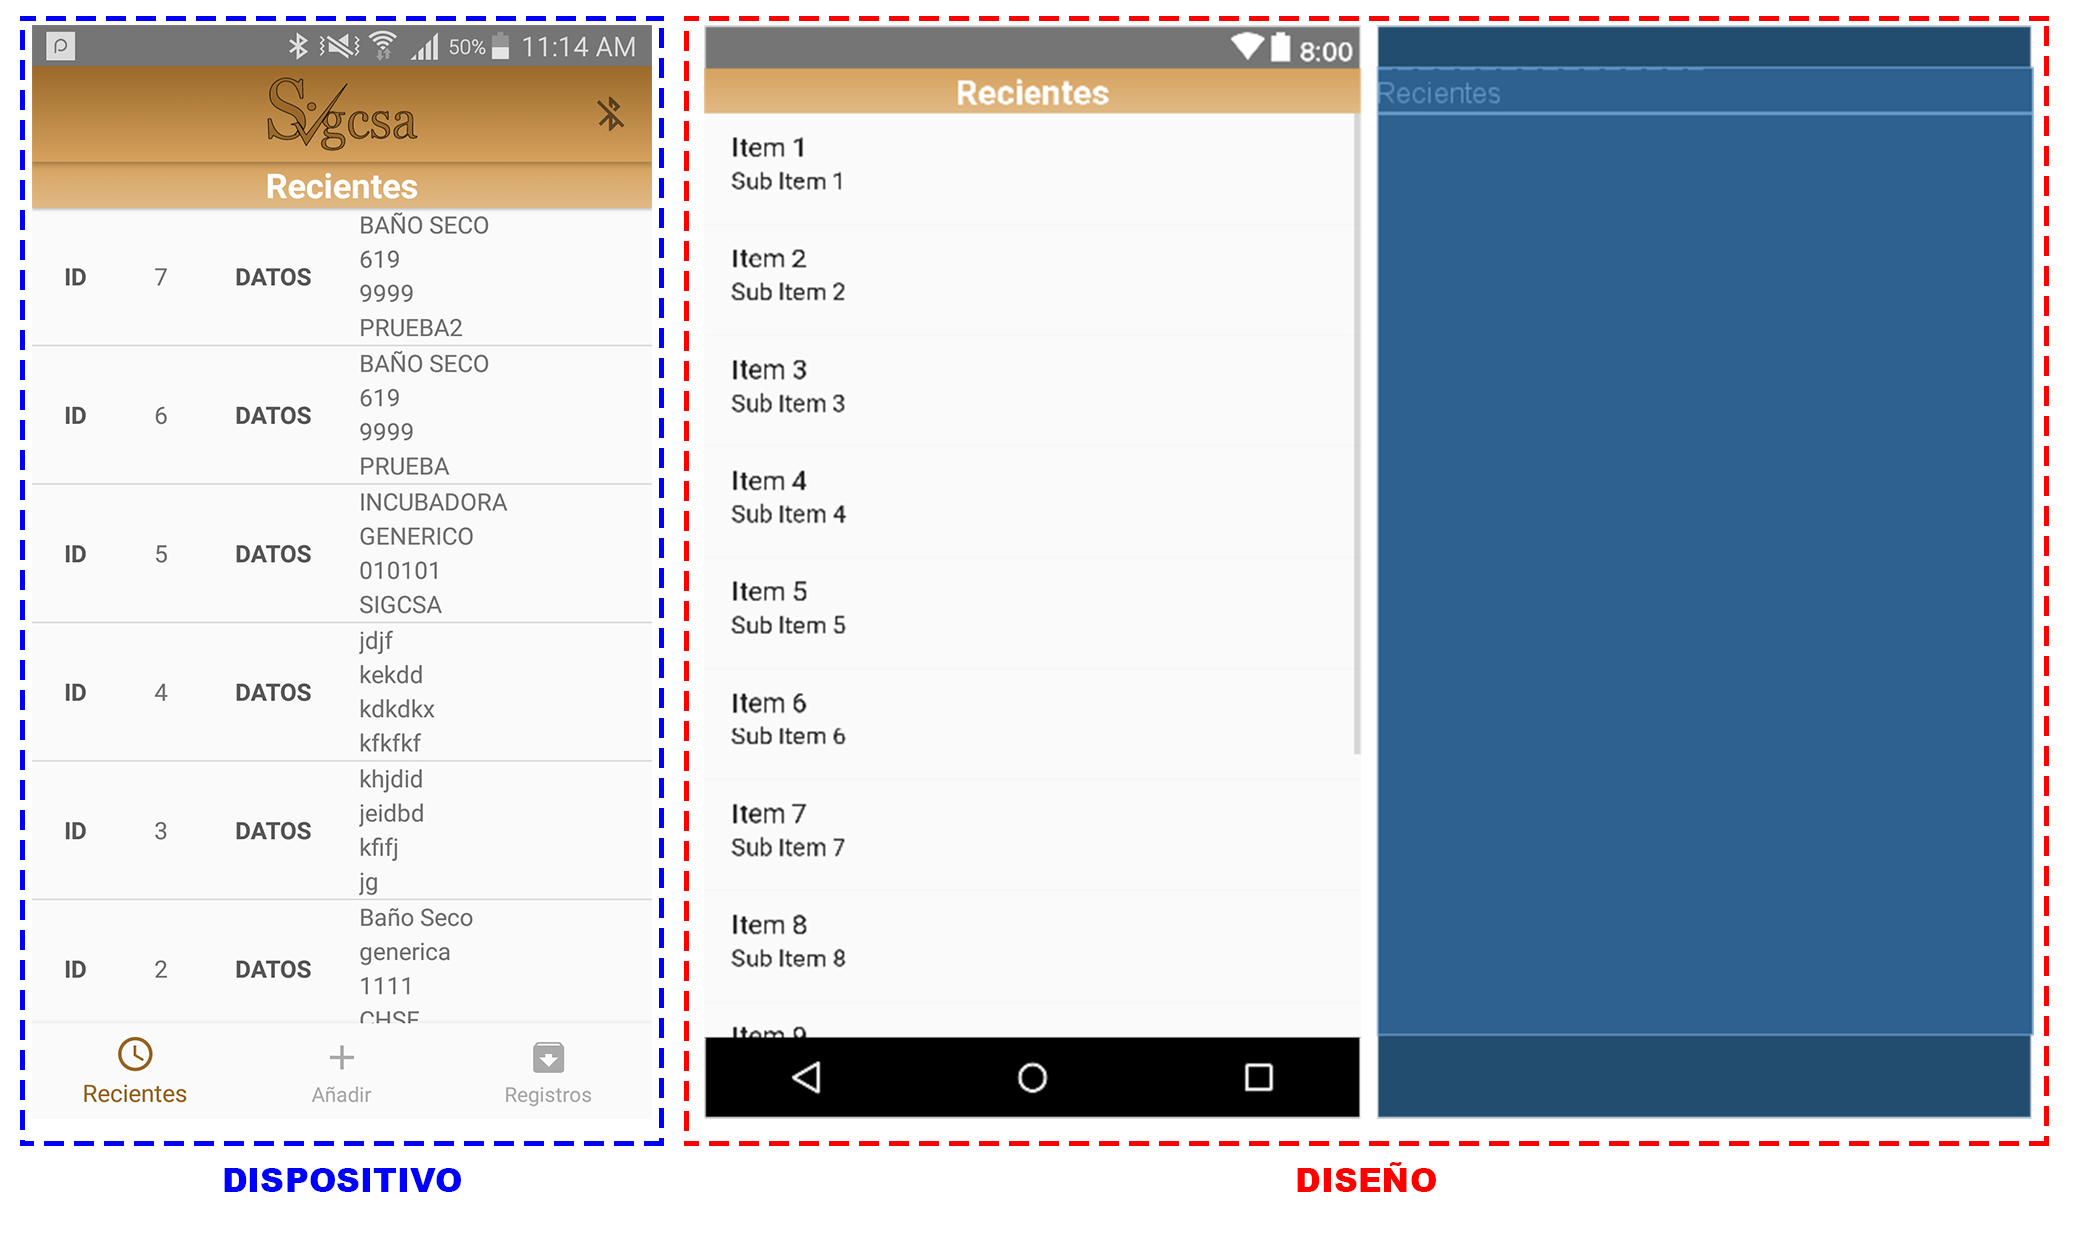
\includegraphics[width=\linewidth]{interfaz3.png}
	\caption{Interfaz del Fragmento Recientes en la aplicación y durante el diseño}
\end{figure}

\par \noindent
Al iniciar la aplicación, se inicia la actividad principal y el valor programado por defecto del "BottonNavegationView" es "Recientes"; por lo que, se procede a visualizar el fragmento recientes en la actividad principal. Un fragmento define una parte distinta del comportamiento de una actividad, incluida la interfaz de usuario asociada. Tiene su propio ciclo de vida que es similar al de la actividad y puede existir junto con otros fragmentos que están integrados en la actividad. Mientras se está ejecutando una actividad, puede agregar y eliminar fragmentos e incluir cada fragmento en una pila posterior administrada por la actividad, lo que permite al usuario navegar hacia atrás a través de los estados de los fragmentos, sin abandonar la actividad\cite{androidapp}. Esta compuesto solamente por 3 componentes. 

\par \noindent
El componente principal es el "layout" que contiene los otros dos elementos que hacen la interfaz del usuario. Recordemos que es importante que los elementos de un fragmento se encuentren dentro de un "layout" ya que es es mas sencillo importar un layout a la actividad principal que todos los componentes por separado. El segundo componente es un "textview" su unico objetivo es el de mostrar texto en la aplicación; sin embargo, puede ser utilizado para indicar al usuario partes de la interfaz. El "textview" despliega el texto "Recientes" y tiene un fondo similar al "toolbar" de la aplicación, esto es para brindar uniformidad en los colores de la aplicación. 

\par \noindent
El ultimo elemento es un "ListView" es un componente especial porque podemos agregarle elementos de forma dinamica como una lista, podemos definirle la interfaz de sus elementos y cada elemento de la lista puede actuar como un botón para iniciar otra actividad. Es un elemento muy versátil e indispensable cuando trabajamos con bases de datos o cuando necesitamos ordenar información importante al usuario.

\begin{figure}[H]
	\centering
	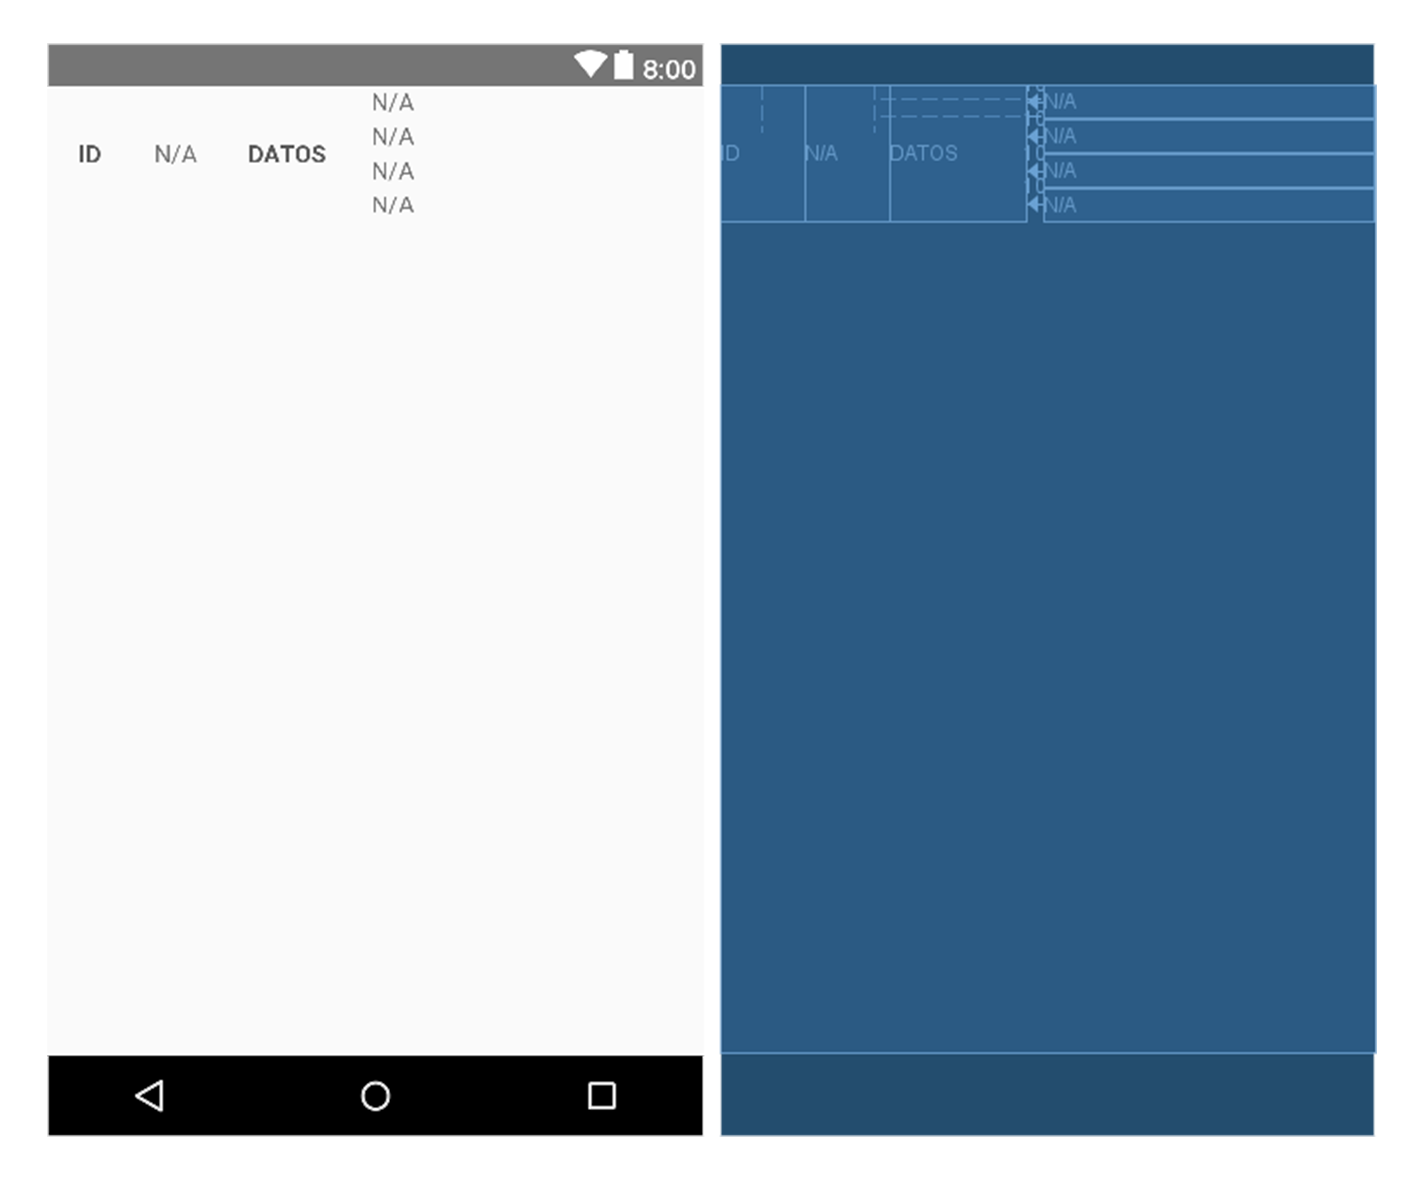
\includegraphics[width=0.5\linewidth]{interfaz4.png}
	\caption{Diseño de interfaz para "ListView" del fragmento recientes y registros}
\end{figure}

\par \noindent
El objetivo de este fragmento es el de mostrar las mediciones realizadas recientemente. Específicamente las ultimas 10 mediciones realizadas en nuestra aplicación. Mas adelante entraremos en detalle a lo que pasa cuando seleccionamos una de las mediciones mostradas en el "ListView". No obstante primero debemos saber como ingresamos datos al fragmento recientes. 

\subsubsection{Fragmento Añadir}

\begin{figure}[H]
	\centering
	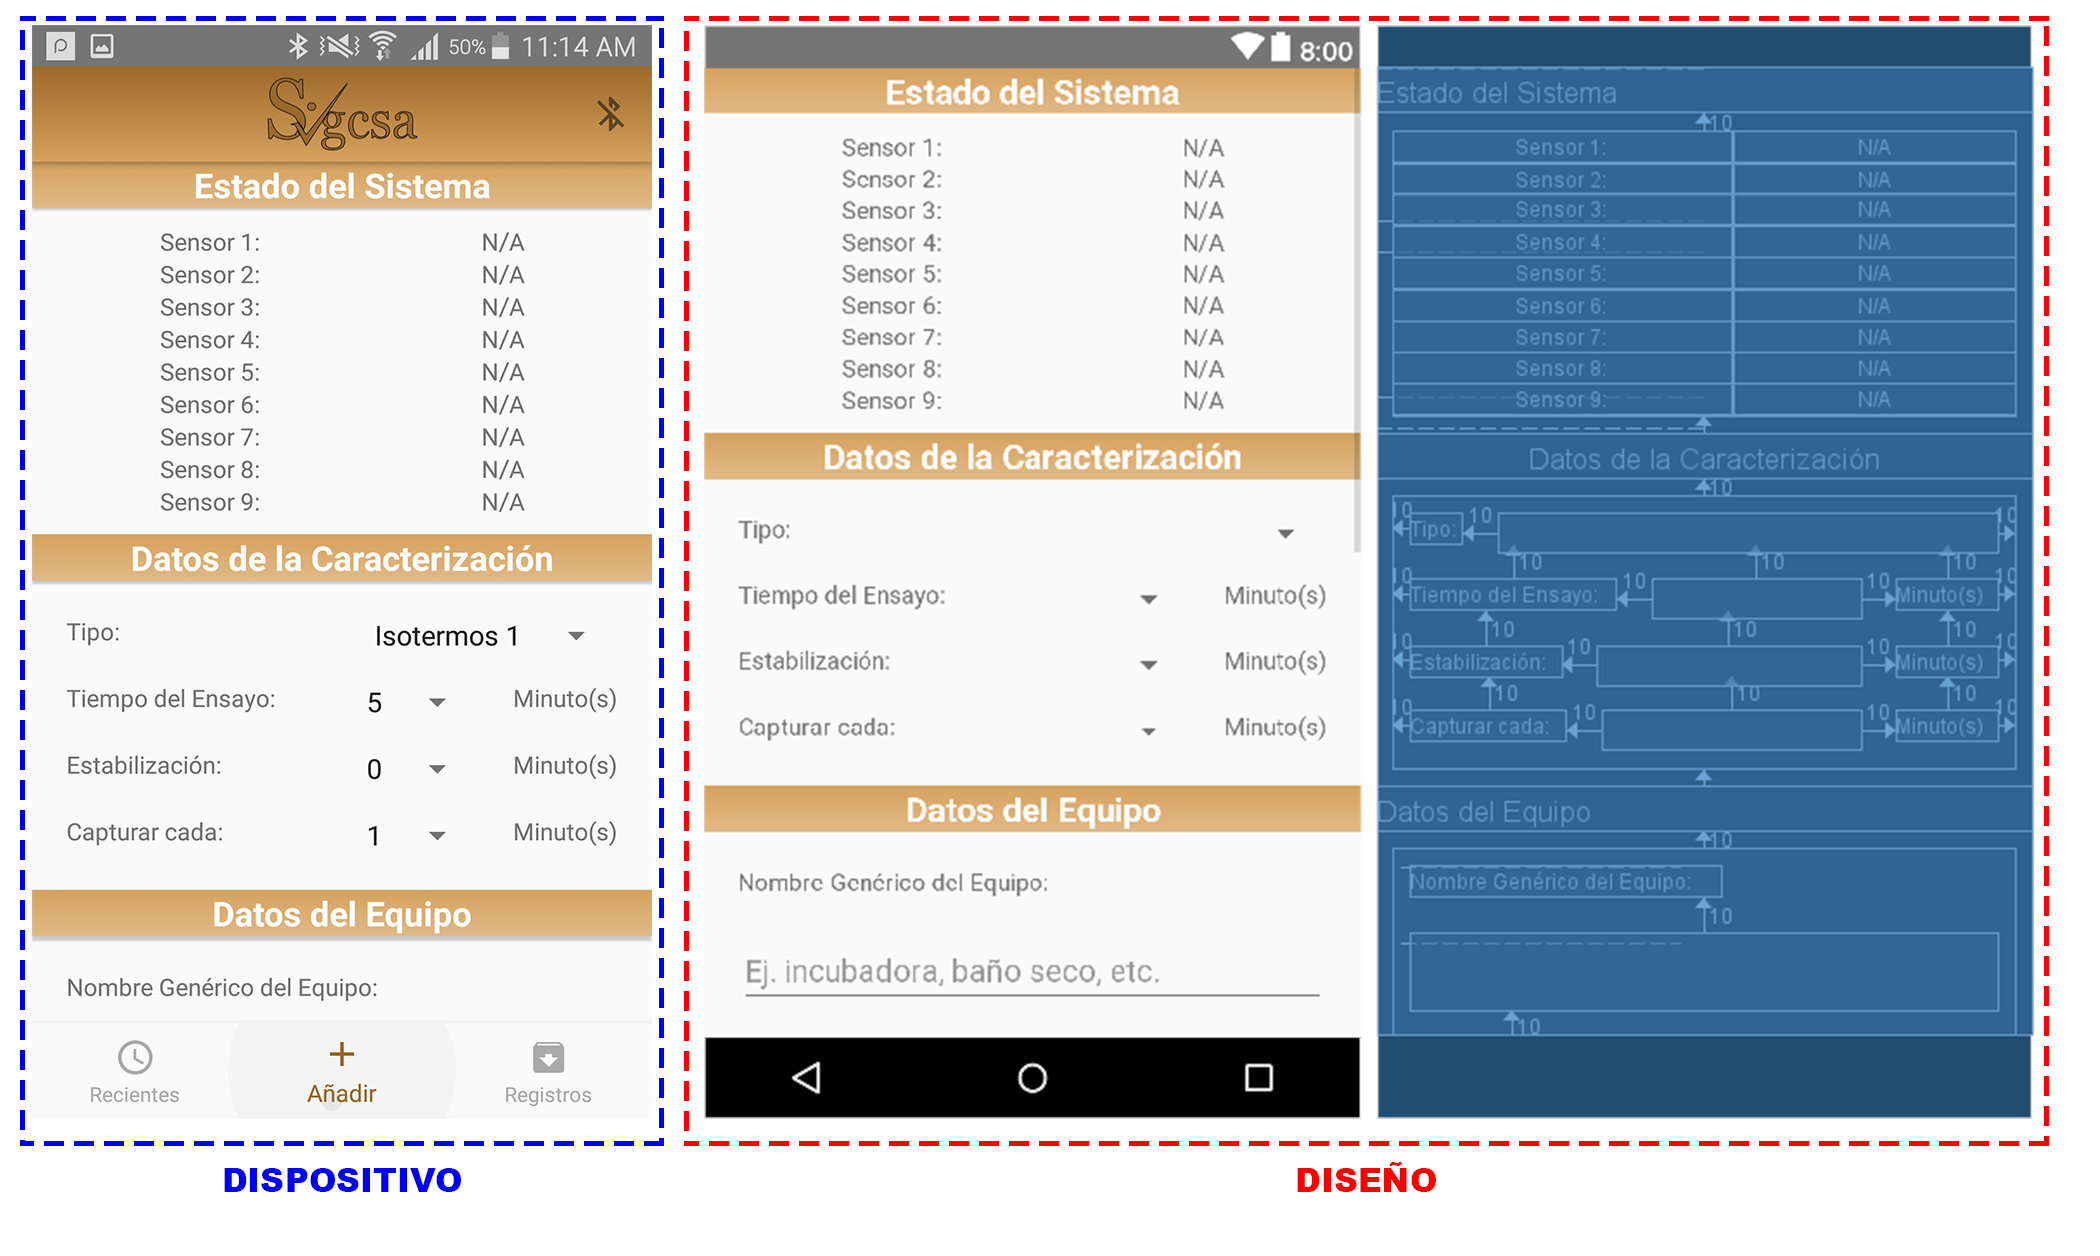
\includegraphics[width=\linewidth]{interfaz5.png}
	\caption{Interfaz del Fragmento Añadir en la aplicación y durante el diseño, parte 1}
\end{figure}

\par 
Facilmente el fragmento añadir es la interfaz mas compleja de este proyecto. El "Layout" utilizado para esta interfaz es un "ScrollView" el cual basicamente es un contenedor con caracterizaticas de desplazamiento vertical. El "ScrollView" es utilizado debido a que todos los elementos de la interfaz no caben en una pantalla promedio de un smartphone. Dentro del "ScrollView" encontramos un "Layout" específicamente un "RelativeLayout" el cual permite un manejo eficiente de los elementos que conforman la interfaz del usuario. 

\par \noindent
El fragmento añadir se divide en 3 secciones. Al inicio el "Estado del Sistema", seguido de  "Datos de la Caracterización" y "Datos del Equipo". Estas secciones son dividas por un simple texto con fondo; con el objetivo de mantener la aplicación fluida al usuario.

\begin{figure}[H]
	\centering
	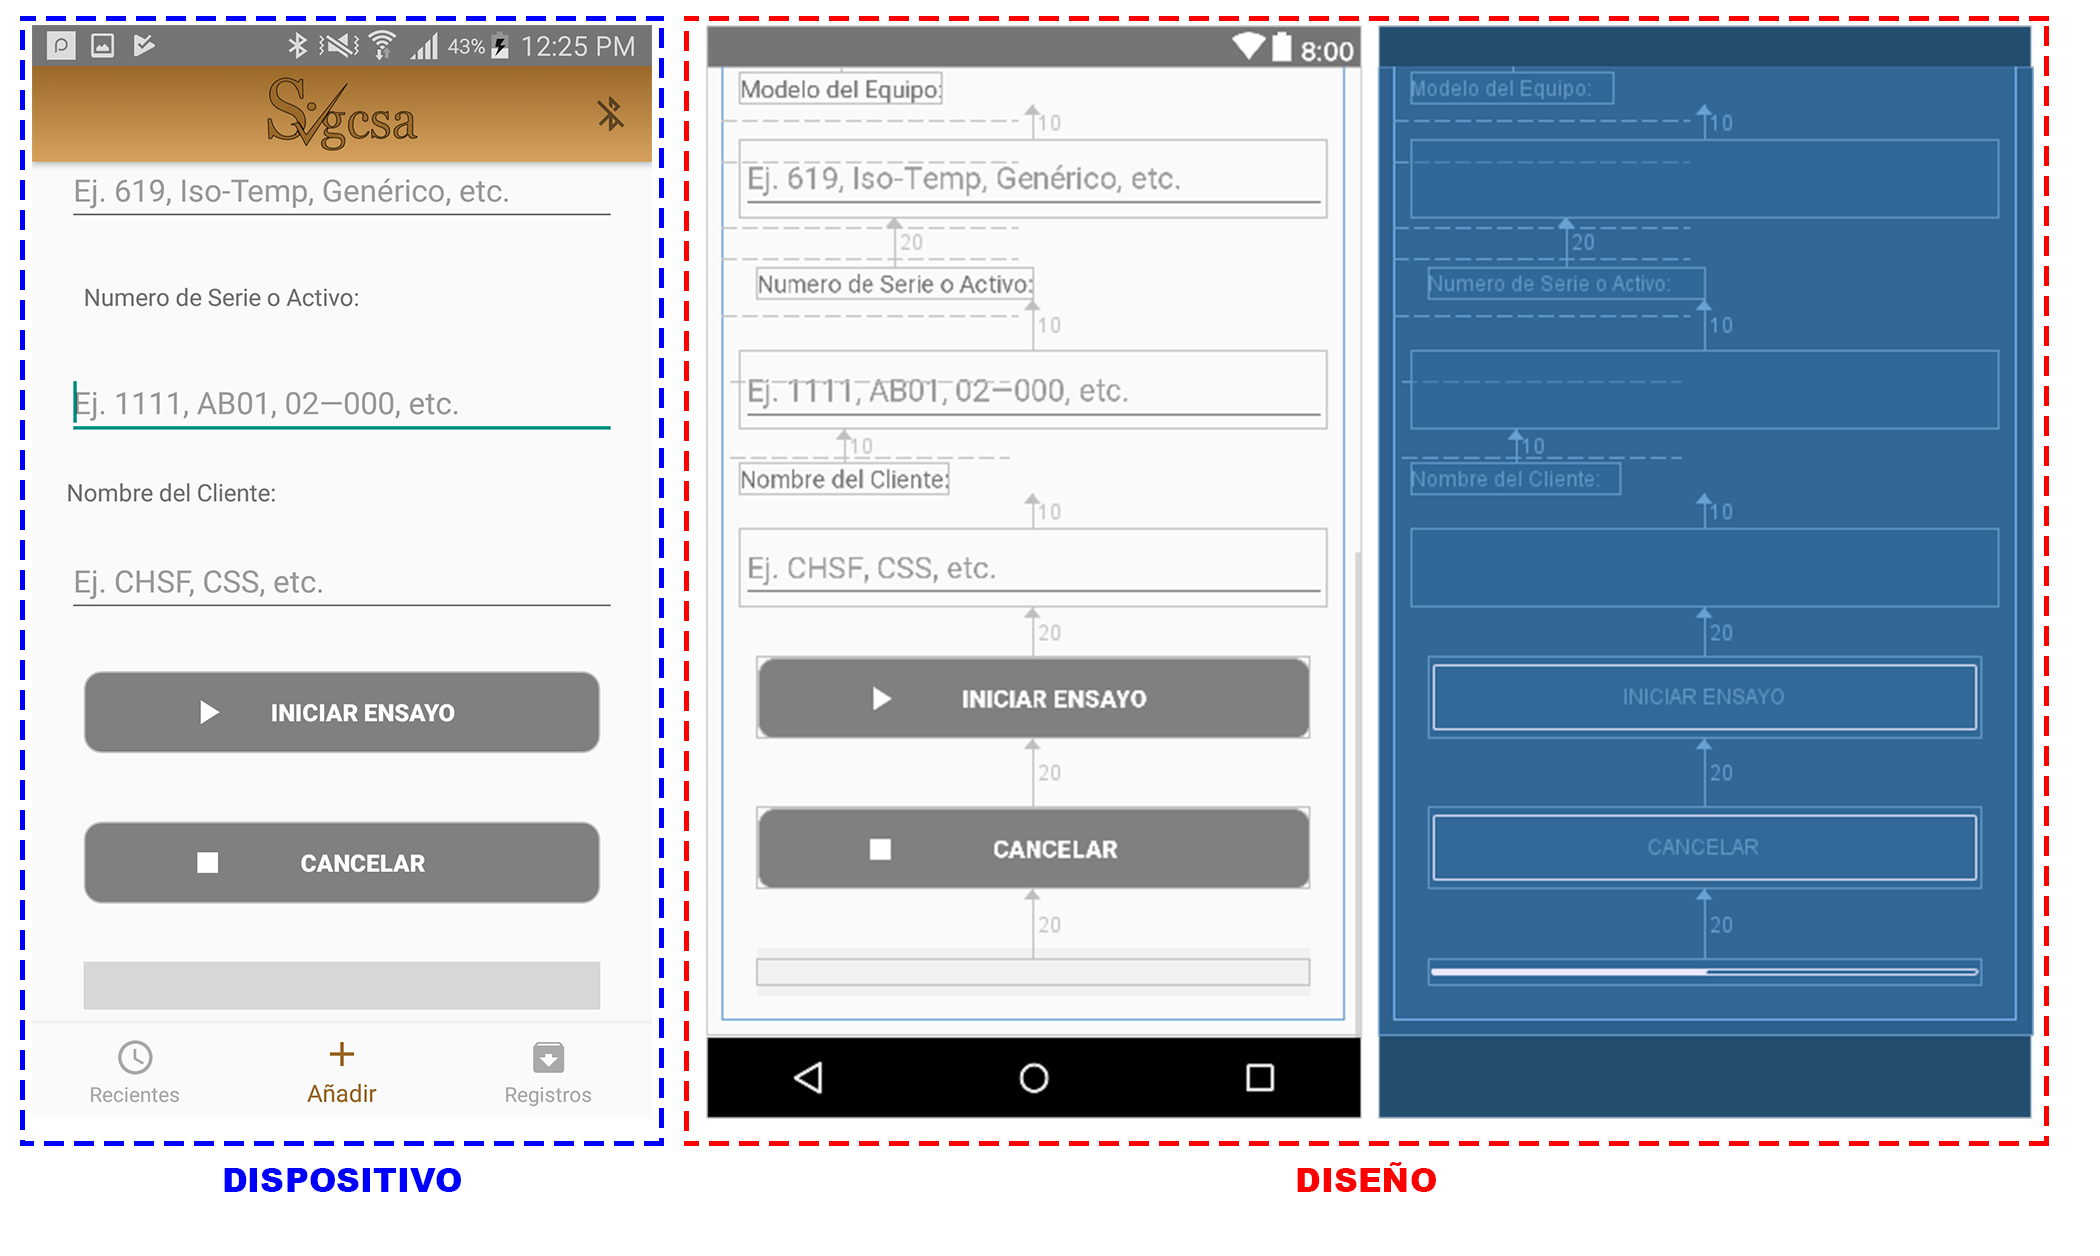
\includegraphics[width=\linewidth]{interfaz6.png}
	\caption{Interfaz del Fragmento Añadir en la aplicación y durante el diseño, parte 2}
\end{figure}

\par \noindent
La sección "Estado del Sistema" contiene los textos que visualizaran las temperaturas de los prototipos; ver imagen 4.13, una vez sea establecida la comunicación por bluetooth. A la izquierda es una guía del numero de sonda o prototipo y a la derecha se encuentra el texto "N/A"; sin embargo, este valor cambiara a la temperatura actual obtenida por su respectivo prototipo y en caso tal de no recibir una lectura se mantendra en el texto "N/A".

\par \noindent
La sección "Datos de la Caracterización" contiene los parametros que definira el usuario para determinar las características de la medición o ensayo. En la imagen 4.13 podemos observar que esta sección consta de 4 casillas donde el usuario puede elegir opciones predeterminas.

\par \noindent
En las opciones de tipo hay 3 opciones: Isotermos 1, Isotermos 2 y Calibración con Patrón. Según el capítulo 3 donde se analizaron los procesos a automatizar podemos notar que los medios Isotermos 1 necesitan de 9 termometros; mientras que, Isotermos 2 de 4 termómetros. Al saber esto debemos tener una interfaz dinamica; la cual dependiendo del tipo de ensayo que se seleccione muestre unicamente la cantidad de prototipos que necesitaremos. 

\begin{figure}[H]
	\centering
	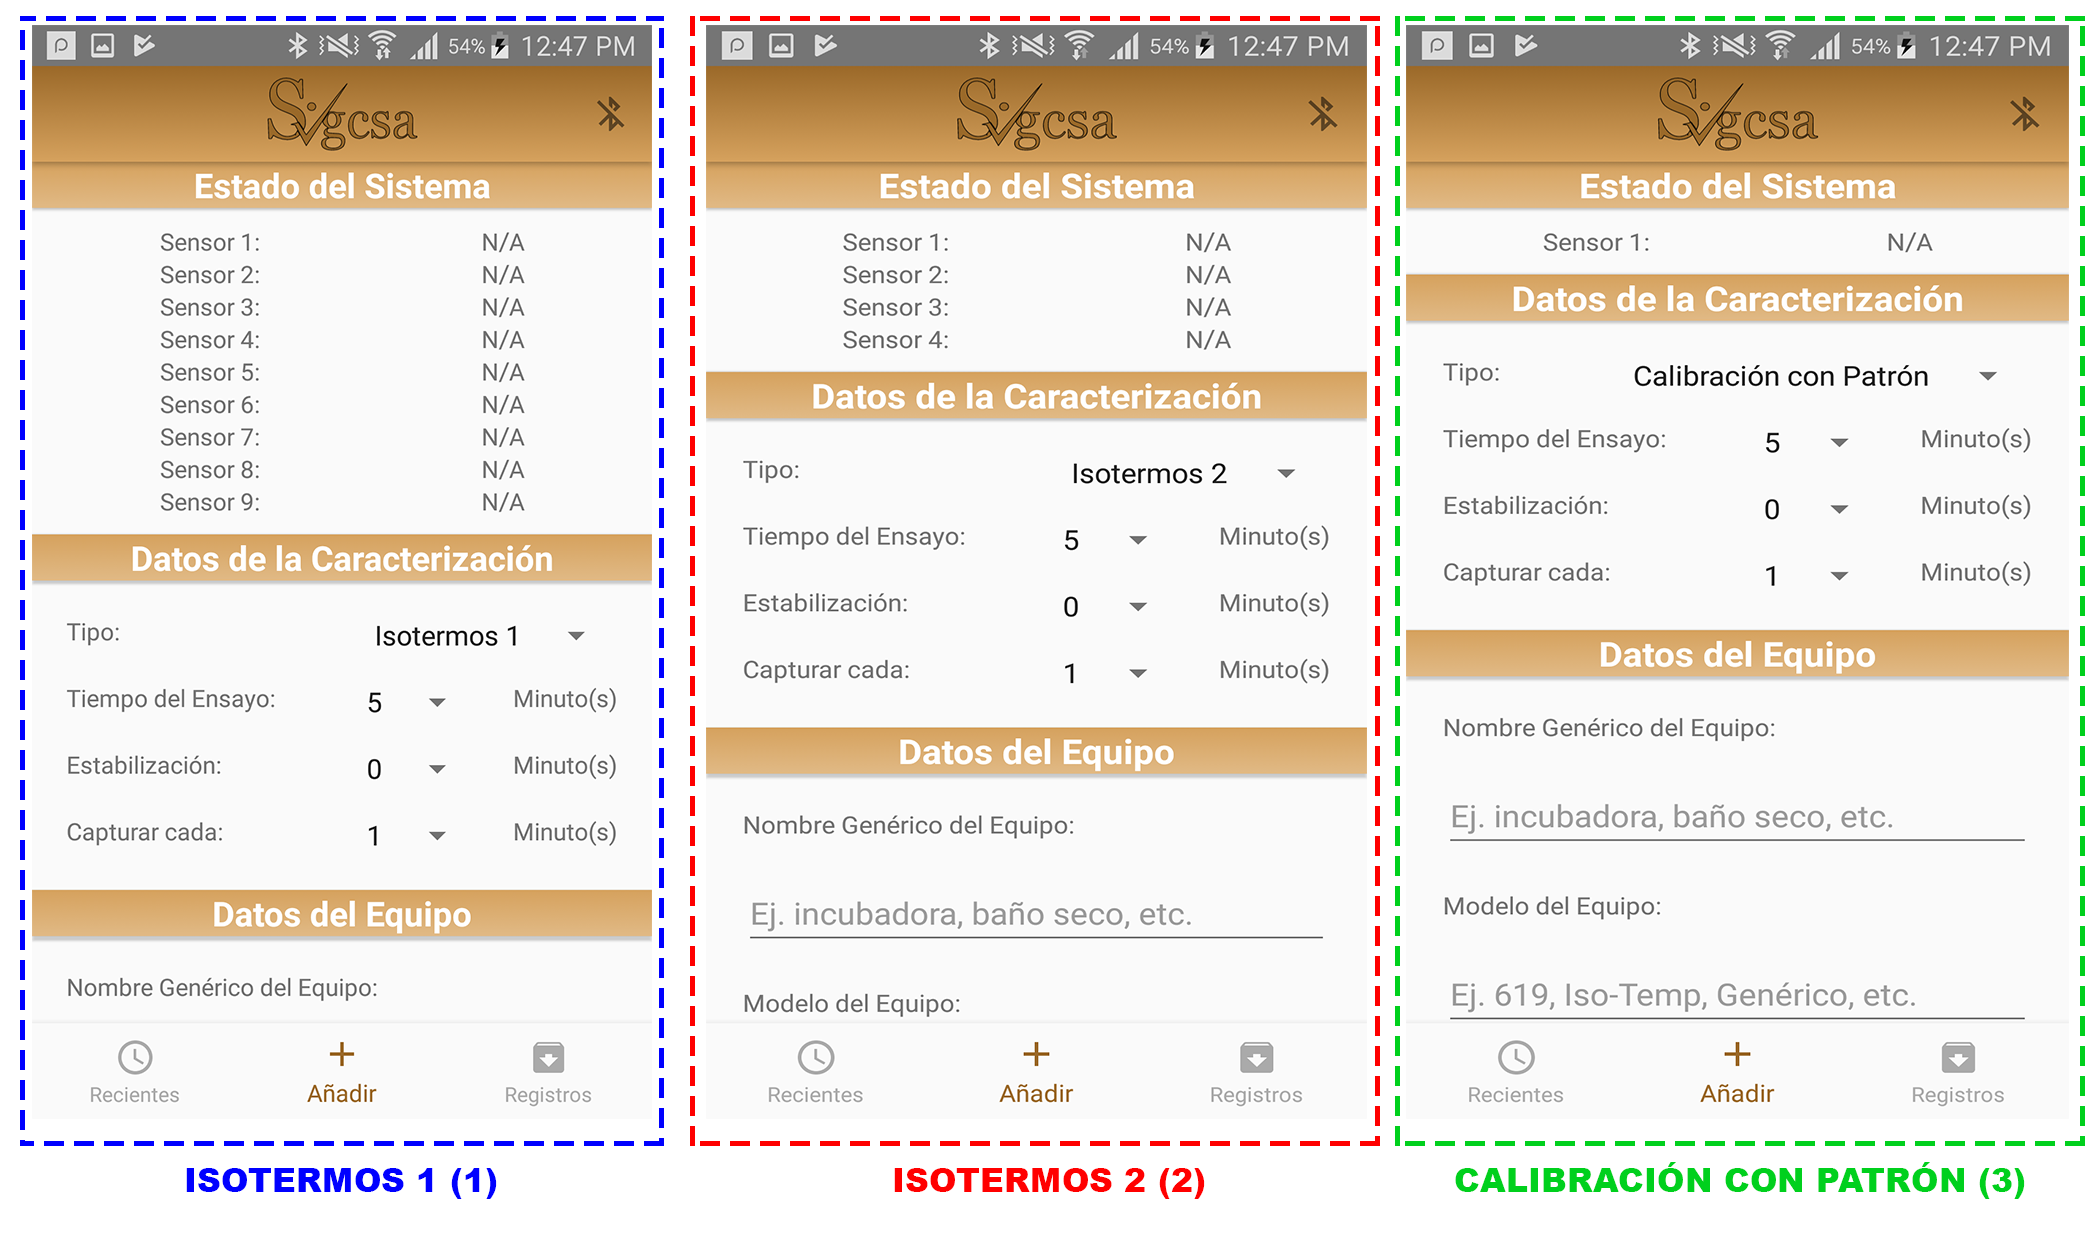
\includegraphics[width=\linewidth]{interfaz7.png}
	\caption{Dependiendo de la opción seleccionada, se ajustan los textos en la sección de "Estado del Sistema"}
\end{figure}

